\section{BGK, AWBS, and Fokker-Planck models in local diffusive regime}
\label{sec:DiffusiveKinetics}

We can try to find an~approximate solution while using the~first term of
expansion in $\mfpe$ and $mu$as
\begin{equation}
  \tilde{f}(z, \vmag, \mu) = f^0(z, \vmag) + f^1(z, \vmag) \mfpei(\vmag)\mu .
  \label{eq:f_approximation}
\end{equation}


\subsection{The~BGK local diffusive electron transport}
\label{sec:BGKDiffusiveRegime}

\begin{multline}
  \mu\left(\pdv{f}{z} + \frac{\tEz}{\vmag}\pdv{f}{\vmag}\right) 
  + \frac{\tEz(1-\mu^2)}{\vmag^2}\pdv{f}{\mu}
  = \\ 
  \frac{f - \fM}{\mfpe}
  + \frac{1}{2}\left(\frac{1}{\mfpei} + \frac{1}{2\mfpe}\right)
  \pdv{}{\mu}(1 - \mu^2)\pdv{f}{\mu} ,
  \label{eq:OOE_AWBS_model_1D}
\end{multline}

\begin{eqnarray}
  f^0 &=& \fM + \frac{1}{\vmag}f^1 \Zbar\mfpei^2 ,
  \label{eq:BGK_f0} \\
  f^1 &=& - \frac{\Zbar}{\Zbar+1}
  \left[ \pdv{f^0}{z} + \frac{\tilde{E}_z}{\vmag}\pdv{f^0}{\vmag} \right] , 
  \label{eq:BGK_f1}
\end{eqnarray}
\begin{equation}
  f = \fM - \frac{\Zbar}{\Zbar+1}
  \left[\frac{1}{\rho}\pdv{\rho}{z} + 
  \left( \frac{\vmag^2}{2 \vth^2} - \frac{3}{2}\right)
  \frac{1}{T}\pdv{T}{z} - \frac{\tilde{E}_z}{\vth^2} \right]\fM \mfpei \mu , 
  \nonumber
\end{equation}
\begin{equation}
  \vect{j} \equiv \qe \int_0^{\infty}\int_{4\pi} \vmag \vn f 
  \, \dI\vn~\vmag^2~\dI\vmag 
  = \vect{0}  \longrightarrow
  \tE = \vth^2\left(\frac{\nabla\rho}{\rho} + \frac{5}{2}\frac{\nabla T}{T} 
  \right) ,
  \label{eq:zero_current}
\end{equation}
\begin{equation}
  f = \fM - \frac{\Zbar}{\Zbar+1}
  \left( \frac{\vmag^2}{2 \vth^2} - 4\right)
  \frac{1}{T}\pdv{T}{z}\fM \mfpei \mu , 
  \nonumber
\end{equation}

\begin{comment} % BGK appendix
\begin{multline}
  \vmag\vn\cdot\nabla f + \tE\cdot\vn \pdv{f}{\vmag} 
  + \frac{\tE\cdot\vect{e}_\theta}{\vmag}\pdv{f}{\theta}
  + \frac{\tE\cdot\vect{e}_\phi}
  {\vmag\sin(\theta)}\pdv{f}{\phi}
  =\\
  \vmag\frac{\left(\fM - f\right)}{\lambda^e} 
  + \frac{\vmag}{2 \lambda^{ei}} 
  \left(\pdv{}{\mu}\left((1 - \mu^2)\pdv{f}{\mu}\right)
  + \frac{1}{\sin^2(\theta)}\frac{\partial^2f}{\partial\phi^2} \right) ,
  \label{eq:BGK_spherical}
\end{multline}
where $\mu = \cos(\theta)$, $\mfpe$ is the~electron-electron mean free path, and
$\mfpei$ is the~electron-ion mean free path. We also approximate
$\mfpe = \Zbar \mfpei$.

%We can try to find an~approximate solution while using the~first term of
%expansion in $\mfp$, $\cos(\phi)$, $\sin(\phi)$, $\sin(\theta)$, and $\fM$ as
%\begin{equation}
%  f = f^0 + f^1 \mfp\fM\cos(\phi) + f^2 \mfp\fM\sin(\phi)\sin(\theta),
%  \label{eq:f_approximation}
%\end{equation}
Clearly, $\pdv{\tilde{f}}{\theta} = 0$, and if $\tB = \tilde{B}_z\vect{e}_z$, 
there is no effect of magnetic field. We also assume, that 
$\nabla f = \pdv{f}{z}\vect{e}_z$ and appropriately 
$\tE = \tilde{E}_z\vect{e}_z$.
From the~orientation of the~Cartesian basis vectors and spherical 
basis vectors, one can find $\tE\cdot\vn = \tilde{E}_z \cos(\phi) = \mu$ and
$\tE\cdot\vect{e}_\phi = -\tilde{E}_z\sin(\phi)$. As a~result, the~analyzed
BGK equation reads
\begin{multline}
  \mu\pdv{}{z}\left( f^0 + f^1 \mfpei\mu \right) 
  + \frac{1}{\vmag} \left[ \tilde{E}_z\mu \pdv{}{\vmag} 
  \left( f^0 + f^1 \mfpei\mu \right) 
  - \frac{\tilde{E}_z\sin(\phi)}{\vmag}\pdv{}{\phi} 
  \left( f^0 + f^1 \mfpei\mu \right)
  \right] 
  =\\
  \frac{\left(\fM - \left( f^0 + f^1 \mfpei\mu \right) \right)}{\mfpe} 
  + \frac{1}{2 \mfpei}\pdv{}{\mu}\left((1 - \mu^2)
  \pdv{}{\mu}\left( f^0 + f^1 \mfpei\mu \right) \right) ,
  \label{eq:BGK_spherical}
\end{multline}

\begin{multline}
  \mu\pdv{f^0}{z} + \mu^2 \pdv{}{z}\left(f^1 \mfpei \right)
  + \frac{\tilde{E}_z}{\vmag} \left[ \mu \pdv{f^0}{\vmag} 
  + \mu^2 \pdv{}{\vmag} \left( f^1 \mfpei \right) 
  + \frac{1 - \mu^2}{\vmag}f^1 \mfpei
  \right] 
  =\\
  \frac{\fM - f^0}{\Zbar\mfpei} - \mu \frac{1}{\Zbar}f^1
  - \mu f^1 ,
  \label{eq:BGK_spherical}
\end{multline}
consequently, we have the~following anisotropy expansion 
$\mu^0, \mu^1, \mu^2, ...$ equations
\begin{eqnarray}
  \frac{\fM - f^0}{\Zbar\mfpei} &=& \frac{\tEz}{\vmag^2}f^1 \mfpei , 
  \nonumber \\
  \pdv{f^0}{z} + \frac{\tilde{E}_z}{\vmag}\pdv{f^0}{\vmag} &=& 
  - \frac{1}{\Zbar}f^1 - f^1 , 
  \nonumber \\ 
  \pdv{}{z}\left(f^1 \mfpei \right) 
  + \frac{\tilde{E}_z}{\vmag} \left[\pdv{}{\vmag} \left( f^1 \mfpei \right)
  - \frac{1}{\vmag}f^1 \mfpei \right] &=& 0 , \nonumber
\end{eqnarray}
which lead to the~definitions
\begin{eqnarray}
  f^0 &=& \fM + \frac{1}{\vmag}f^1 \Zbar\mfpei^2 ,
  \label{eq:BGK_f0} \\
  f^1 &=& - \frac{\Zbar}{\Zbar+1}
  \left[ \pdv{f^0}{z} + \frac{\tilde{E}_z}{\vmag}\pdv{f^0}{\vmag} \right] 
  \nonumber \\
  &=& - \frac{\Zbar}{\Zbar+1}
  \left[\frac{1}{\rho}\pdv{\rho}{z} + 
  \left( \frac{\vmag^2}{2 \vth^2} - \frac{3}{2}\right)
  \frac{1}{T}\pdv{T}{z} - \frac{\tilde{E}_z}{\vth^2} \right]\fM 
  %\nonumber \\
  %&=& - \frac{\Zbar}{\Zbar+1}
  %\left( \frac{\vmag^2}{2 \vth^2} - \frac{3}{2} - \alpha\right)
  %\frac{1}{T}\pdv{T}{z}\fM ,
  \label{eq:BGK_f1}
\end{eqnarray}

In order to ensure the~plasma to be quasi-neutral, the~zero-current condition
\begin{equation}
  \vect{j} = \int_0^{\infty}\int_{4\pi} \qe \vmag \vn f 
  \, \dI\vn~\vmag^2~\dI\vmag 
  = \vect{0} ,
  \label{eq:zero_current}
\end{equation}
can be achieved by providing a~consistent electric field in 
\refeq{eq:f_approximation}, i.e.
\begin{equation}
  \tE = \frac{\vth^2~\int_{4\pi} \vn\otimes\vn\cdot \int_0^{\infty} \vmag  
  \fM \frac{\mfp}{\alpha}\left(\frac{\nabla\rho}{\rho} + 
  \left( \frac{\vmag^2}{2 \vth^2} - \frac{3}{2}\right) 
  \frac{\nabla T}{T}\right)
  \vmag^2\, \dI\vmag\, \dI\vn}
  {\int_{4\pi} \vn\otimes\vn\cdot \int_0^{\infty} \vmag  
  \fM \frac{\mfp}{\alpha}\vmag^2\, \dI\vmag\, \dI\vn} ,
\end{equation}
which may be further simplified as
\begin{equation}
  \tE = \frac{\int_0^{\infty} \fM
  \frac{1}{2}\frac{\nabla T}{T}\vmag^9\, \dI\vmag}
  {\int_0^{\infty} \fM \vmag^7\, \dI\vmag} + 
  \vth^2\left(\frac{\nabla\rho}{\rho} - \frac{3}{2}\frac{\nabla T}{T} \right)
  = \vth^2\left(\frac{\nabla\rho}{\rho} + \frac{5}{2}\frac{\nabla T}{T} 
  \right) ,
\end{equation}
where it is worth mentioning, that the~part 
$\fM + \frac{\vmag\mfp}{\alpha} \pdv{f_1}{\vmag}$ of the~distribution
does not contribute to the~current since it is isotropic.
One can write the~quasi-neutral distribution function explicitly 
distinguishing between original part (blue color) and E field correction
(red color) as
\begin{equation}
  f \approx \fM \left(1 - \frac{\mfp}{\alpha}\vn\cdot\left( 
  \textcolor{blue}{
  \frac{\vmag^2}{2 \vth^2} - \frac{3}{2}
  }
  \textcolor{red}{
  - \frac{5}{2}
  }
  \right) \frac{\nabla T}{T} \right) 
  + \frac{\vmag\mfp}{\alpha} \pdv{f_1}{\vmag} .
  \label{eq:f_localized_quasineutral}
\end{equation}
which leads to the~resulting heat flux
\begin{equation}
  \vect{q}_H = \int_{4\pi}\int_0^{\infty} \frac{\me \vmag^2}{2} \vmag \vn f 
  \vmag^2\, \dI\vmag\, \dI\vn = \frac{4\pi}{3}\frac{\me}{2}
  \frac{1}{\alpha \crs\rho}
  \int_0^{\infty} \left( 
  \textcolor{blue}{
  \frac{\vmag^2}{2 \vth^2} - \frac{3}{2}
  }
  \textcolor{red}{
  - \frac{5}{2}
  }
  \right) \vmag^9 \fM\, \dI\vmag \frac{\nabla T}{T} .
  \nonumber
\end{equation} 
Based on the~Gauss integral formula
\begin{equation}
  \int \vmag^{2s+1} \exp\left(-\frac{\vmag^2}{2\vth^2}\right)\, \dI\vmag = 
  \frac{s!~(2 \vth^2)^{s+1}}{2}
  \nonumber 
\end{equation}
and Maxwell-Boltzmann distribution \refeq{eq:MBdistribution} the~heat flux can 
be written as
\begin{equation}
  \vect{q}_H = \frac{4\pi}{3}\frac{\me}{2}\frac{1}{\alpha \crs\rho}
  \frac{\rho}{\vth^3 \left( 2 \pi \right)^{3/2}}
  \frac{4!~2^4 \vth^{10}}{T} \left( 
  \textcolor{blue}{
  5 - \frac{3}{2}
  }
  \textcolor{red}{
  - \frac{5}{2}
  }
  \right) \nabla T 
  = \frac{\me}{\alpha \crs}\frac{128}{\sqrt{2 \pi}}
  \left(\frac{\kB}{\me}\right)^{\frac{7}{2}}T^{\frac{5}{2}} \nabla T .
  \label{eq:Lorentz_flux}
\end{equation} 
In conclusion, equation \refeq{eq:Lorentz_flux} provides nothing else than
the~well known Lorentz approximation heat flux and its nonlinearity $2.5$
in temperature. What is worth mentioning is the~effect of E field 
(quasi-neutrality), which reduces the~flux of about	71.4$\%$ 
(also assuming constant density).


Finally, one can find the~approximate solution
\begin{equation}
  \tilde{f} = \fM - \mfpei\frac{\Zbar}{\Zbar+1}
  \left( \frac{\vmag^2}{2 \vth^2} - \frac{3}{2} - \alpha\right)
  \frac{\vn\cdot\nabla T}{T}\fM .
  \label{eq:BGK_approximate_solution}
\end{equation}
\end{comment} % BGK appendix

\subsection{The~AWBS diffusive electron transport}
\label{sec:AWBSDiffusiveRegime}

\begin{multline}
  \mu\left(\pdv{f}{z} + \frac{\tEz}{\vmag}\pdv{f}{\vmag}\right) 
  + \frac{\tEz(1-\mu^2)}{\vmag^2}\pdv{f}{\mu}
  = \\ 
  \frac{\vmag}{2\mfpe} \pdv{}{\vmag}\left(f - \fM\right) 
  + \frac{1}{2}\left(\frac{1}{\mfpei} + \frac{1}{2\mfpe}\right)
  \pdv{}{\mu}(1 - \mu^2)\pdv{f}{\mu} ,
  \label{eq:OOE_AWBS_model_1D}
\end{multline}

\begin{eqnarray}
  \pdv{}{\vmag}\left( f^0 -\fM\right) &=& \frac{1}{\vmag^2}f^1 \Zbar\mfpei^2 ,
  \label{eq:AWBS_f0} \\
  \frac{\vmag}{\Zbar\mfpei}\pdv{\left(f^1 \mfpei\right)}{\vmag}  
  - \frac{\Zbar + 1}{\Zbar} f^1 &=&
  \pdv{f^0}{z} + \frac{\tilde{E}_z}{\vmag}\pdv{f^0}{\vmag}
  \nonumber 
  %\\  
  %\frac{\vmag}{\Zbar}\pdv{f^1}{\vmag} + \frac{4}{\Zbar}f^1 
  %- \frac{\Zbar + 1}{\Zbar} f^1 &=&
  %\pdv{f^0}{z} + \frac{\tilde{E}_z}{\vmag}\pdv{f^0}{\vmag}
  %\nonumber
\end{eqnarray}

\begin{equation}
  \pdv{f^1}{\vmag} + \frac{1}{\vmag}(3-\Zbar)f^1
  =
  \frac{\Zbar}{\vmag}\left(\frac{1}{\rho}\pdv{\rho}{z} + 
  \left( \frac{\vmag^2}{2 \vth^2} - \frac{3}{2}\right)
  \frac{1}{T}\pdv{T}{z} - \frac{\tilde{E}_z}{\vth^2}\right)\fM .
  \label{eq:AWBS_f1}
\end{equation}

\begin{comment} % AWBS appendix
The~AWBS electron transport equation in 6D reads
\begin{multline}
  \vn\cdot\nabla f + \frac{1}{\vmag} \left[ \tE\cdot\vn \pdv{f}{\vmag} 
  + \frac{\tE\cdot\vect{e}_\phi 
  - \vmag\tB\cdot\vect{e}_\theta}{\vmag}\pdv{f}{\phi}
  + \frac{\tE\cdot\vect{e}_\theta + \vmag\tB\cdot\vect{e}_\phi}
  {\vmag\sin(\phi)}\pdv{f}{\theta} \right] 
  =\\
  \frac{\vmag}{\lambda^e}\pdv{}{\vmag}\left(f - f_M\right) 
  + \left(\frac{1}{\mfpei} + \frac{1}{\mfpe} \right) \frac{1}{2}
  \left(\pdv{}{\mu}\left((1 - \mu^2)\pdv{f}{\mu}\right)
  + \frac{1}{\sin^2(\phi)}\frac{\partial^2f}{\partial\theta^2} \right) ,
  \label{eq:AWBS_spherical}
\end{multline}
where $\mu = \cos(\phi)$, $\mfpe$ is the~electron-electron mean free path, and
$\mfpei$ is the~electron-ion mean free path, and $\mfpe = \Zbar \mfpei$.

We can try to find an~approximate solution while using the~first term of
expansion in $\mfpe$ and $\mu$ as
\begin{equation}
  \tilde{f}(z, \vmag, \mu) = f^0(z, \vmag) + f^1(z, \vmag) \mfpei\mu .
  \label{eq:f_approximation}
\end{equation}
Clearly, $\pdv{\tilde{f}}{\theta} = 0$, and if $\tB = \tilde{B}_z\vect{e}_z$, 
there is no effect of magnetic field. We also assume, that 
$\nabla f = \pdv{f}{z}\vect{e}_z$ and appropriately 
$\tE = \tilde{E}_z\vect{e}_z$.
From the~orientation of the~Cartesian basis vectors and spherical 
basis vectors, one can find $\tE\cdot\vn = \tilde{E}_z \cos(\phi) = \mu$ and
$\tE\cdot\vect{e}_\phi = -\tilde{E}_z\sin(\phi)$. As a~result, the~analyzed
AWBS equation reads
\begin{multline}
  \mu\pdv{}{z}\left( f^0 + f^1 \mfpei\mu \right) 
  + \frac{1}{\vmag} \left[ \tilde{E}_z\mu \pdv{}{\vmag} 
  \left( f^0 + f^1 \mfpei\mu \right) 
  - \frac{\tilde{E}_z\sin(\phi)}{\vmag}\pdv{}{\phi} 
  \left( f^0 + f^1 \mfpei\mu \right)
  \right] 
  =\\
  \frac{\vmag}{\mfpe}\pdv{}{\vmag}
  \left(\left( f^0 + f^1 \mfpei\mu \right) -\fM\right)
  + \frac{\Zbar +1}{2 \mfpei \Zbar}\pdv{}{\mu}\left((1 - \mu^2)
  \pdv{}{\mu}\left( f^0 + f^1 \mfpei\mu \right) \right) ,
  \label{eq:AWBS_spherical}
\end{multline}

\begin{multline}
  \mu\pdv{f^0}{z} + \mu^2 \pdv{}{z}\left(f^1 \mfpei \right)
  + \frac{\tilde{E}_z}{\vmag} \left[ \mu \pdv{f^0}{\vmag} 
  + \mu^2 \pdv{}{\vmag} \left( f^1 \mfpei \right) 
  + \frac{1 - \mu^2}{\vmag}f^1 \mfpei
  \right] 
  =\\
  \frac{\vmag}{\Zbar\mfpei}\pdv{}{\vmag}
  \left( f^0 -\fM\right)
  + \mu\frac{\vmag}{\Zbar\mfpei}\pdv{\left(f^1 \mfpei\right)}{\vmag} 
  - \mu \frac{\Zbar + 1}{\Zbar}f^1 ,
  \label{eq:AWBS_spherical}
\end{multline}
consequently, we have the~following anisotropy expansion 
$\mu^0, \mu^1, \mu^2, ...$ equations
\begin{eqnarray}
  \frac{\vmag}{\Zbar\mfpei}\pdv{}{\vmag}
  \left( f^0 -\fM\right) &=& \frac{\tEz}{\vmag^2}f^1 \mfpei , 
  \nonumber \\
  \pdv{f^0}{z} + \frac{\tilde{E}_z}{\vmag}\pdv{f^0}{\vmag} &=& 
  \frac{\vmag}{\Zbar\mfpei}\pdv{\left(f^1 \mfpei\right)}{\vmag}  
  - \frac{\Zbar + 1}{\Zbar} f^1 , 
  \nonumber \\ 
  \pdv{}{z}\left(f^1 \mfpei \right) 
  + \frac{\tilde{E}_z}{\vmag} \left[\pdv{}{\vmag} \left( f^1 \mfpei \right)
  - \frac{1}{\vmag}f^1 \mfpei \right] &=& 0 , \nonumber
\end{eqnarray}
which lead to the~definitions
\begin{eqnarray}
  \pdv{}{\vmag}\left( f^0 -\fM\right) &=& \frac{1}{\vmag^2}f^1 \Zbar\mfpei^2 ,
  \label{eq:AWBS_f0} \\
  \frac{\vmag}{\Zbar\mfpei}\pdv{\left(f^1 \mfpei\right)}{\vmag}  
  - \frac{\Zbar + 1}{\Zbar} f^1 &=&
  \pdv{f^0}{z} + \frac{\tilde{E}_z}{\vmag}\pdv{f^0}{\vmag}
  \nonumber \\  
  \frac{\vmag}{\Zbar}\pdv{f^1}{\vmag} + \frac{4}{\Zbar}f^1 
  - \frac{\Zbar + 1}{\Zbar} f^1 &=&
  \pdv{f^0}{z} + \frac{\tilde{E}_z}{\vmag}\pdv{f^0}{\vmag}
  \nonumber \\
  \pdv{f^1}{\vmag} + \frac{1}{\vmag}(3-\Zbar)f^1
  &=&
  \frac{\Zbar}{\vmag}\left(\frac{1}{\rho}\pdv{\rho}{z} + 
  \left( \frac{\vmag^2}{2 \vth^2} - \frac{3}{2}\right)
  \frac{1}{T}\pdv{T}{z} - \frac{\tilde{E}_z}{\vth^2}\right)\fM .
  \label{eq:AWBS_f1}
\end{eqnarray}
\end{comment} % AWBS appendix

\subsection{The~Fokker-Planck diffusive electron transport}
\label{sec:FPDiffusiveRegime}
\begin{equation}
  \vtwoh = \sqrt{\frac{2 \kB T}{\me}} = 1 / j,
  \nonumber
\end{equation}
\begin{eqnarray}
  A &=& -\frac{\me^2 \vtwoh^2 \tE}{2 \pi e^4 n_e \lnc} = - \frac{m E}{2\pi j^2 e^3 n_e \lnc}
  , \nonumber \\
  B &=& \frac{\me^2 \vtwoh^4 |\nabla T|}{2 \pi e^4 n_e \lnc T} = \frac{2 \kB^2 T |\nabla T|}{\pi e^4 n_e \lnc}
  , \nonumber
\end{eqnarray}
\begin{equation}
  \frac{A}{B} = - \frac{|\tE| T}{\vtwoh^2 |\nabla T|} ,
  \nonumber
\end{equation}
\begin{equation}
  \tE = -\frac{3}{2}\frac{\vtwoh^2}{2}\frac{\gamma_T}{\gamma_E}
  \frac{\nabla T}{T} ,
  \nonumber
\end{equation}
From Eq. (24) CSR, we can write the~form of $f_1$ including both $\nabla T$ 
and $\tE$ effects as
\begin{equation}
  f_1(\vmag, \theta) = \cos(\theta) \frac{B}{\Zbar}\left( d_T(\vmag/\vtwoh) 
  + \frac{A}{B} d_E(\vmag/\vtwoh) \right) \fM(\vmag)  ,
  \nonumber
\end{equation}
where in the~case of vanishing current one gets
\begin{equation}
  \frac{A}{B} = \frac{3}{2}\frac{\gamma_T}{2 \gamma_E} ,
  \nonumber
\end{equation}
i.e.
\begin{equation}
  f_1(\vmag, \theta) = \cos(\theta) \frac{\me^2}{4 \pi e^4\lnc} 
  \frac{\vtwoh^4}{\Zbar}\left( 2 d_T(\vmag/\vtwoh) 
  + \frac{3}{2}\frac{\gamma_T}{\gamma_E} d_E(\vmag/\vtwoh) \right) 
  \frac{\fM(\vmag)}{n_e}\frac{\nabla T}{T}  ,
  \label{eq:f1_SH}
\end{equation}
where $d_T(x) = \Zbar D_{T}(x) / B$ and $d_E(x) = \Zbar D_{E}(x) / A$ 
are represented by numerical values in TABLE I and TABLE II in 
\cite{SH_PR1953}, respectively. 
In the~case of high $\Zbar$ limit, $\gamma_T \rightarrow 1$,
$\gamma_E \rightarrow 1$, $d_E(x) = x^4$, and $d_T(x) = x^4 (2.5 - x^2)/2$
\cite{SH_PR1953}, which leads to the~standard Lorentz gas model
\begin{equation}
   f_1(\vmag, \theta) = \cos(\theta) \frac{\me^2}{4 \pi e^4\lnc} 
  \frac{\vmag^4}{\Zbar}\left( 4 - \frac{\vmag^2}{\vtwoh^2} \right) 
  \frac{\fM(\vmag)}{n_e}\frac{\nabla T}{T}  ,
  \label{eq:f1_Lorentz} 
\end{equation}

\cite{Rosenbluth_PR1957}, \cite{Longmire_1963}, \cite{Shkarofsky_1966}

\subsection{Summary of BGK, AWBS, and Fokker-Planck diffusion}
\label{sec:SummaryDiffusiveKinetics}

\begin{figure}[tbh]
  \begin{center}
    \begin{tabular}{c}
      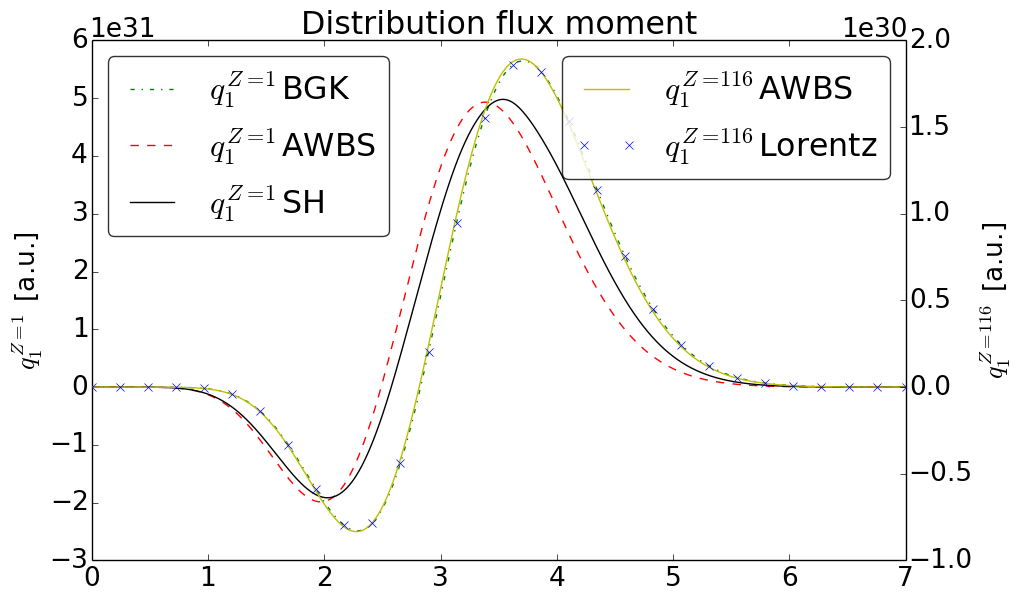
\includegraphics[width=1.0\textwidth]{q1s.png}
    \end{tabular}
  \caption{  
  The~flux velocity moment of the~anisotropic part of the~electron distribution 
  function in low $Z=1$ and high $Z=116$ plasmas in diffusive regime.}
  \end{center}
  \label{fig:q1s_summary}
\end{figure}

\begin{table}
\begin{center}
  \begin{tabular}{c|ccccc}
    \hline\hline\\
    %$\Zbar$ & $1$ & $2$ & $4$ & $16$ & $\infty$ \\\\
    & $\,\Zbar=1\,$ & $\,\Zbar=2\,$ & $\,\Zbar=4\,$ & $\,\Zbar=16\,$ & $\,\Zbar=116\,$ \\\\
    \hline\\
    $\bar{\Delta}\vect{q}_{AWBS}$ & 0.057 & 0.004 & 0.038 & 0.049 & 0.004 \\\\
    \hline\hline
  \end{tabular}
  \caption{
  Relative error $\bar{\Delta}\vect{q}_{AWBS} = 
  |\vect{q}_{AWBS} - \vect{q}_{SH}| / \vect{q}_{SH}$ of the~AWBS
  kinetic model equation \refeq{eq:AWBS_model} showing the~discrepancy 
  (maximum around 5$\%$) with respect to the~original solution of 
  the~heat flux given by Spitzer and Harm \cite{SH_PR1953}.
  }
\end{center}
\label{tab:qAWBS}
\end{table}

